\documentclass[12pt, a4paper]{article}

% ── PAQUETES ─────────────────────────────────────────────────
% Los paquetes amplían las capacidades de LaTeX.
% Se cargan en el "preámbulo" (antes de \begin{document}).

\usepackage[utf8]{inputenc}       % Permite tildes y ñ
\usepackage[spanish]{babel}       % Idioma español (guiones, fechas, etc.)
\usepackage{geometry}             % Control de márgenes
\usepackage{graphicx}             % Para insertar imágenes
\usepackage{setspace}             % Control de interlineado
\usepackage{hyperref}             % Links clicables (índice, URLs)
\usepackage{xcolor}               % Colores personalizados
\usepackage{listings}
\usepackage{tcolorbox}
\usepackage{amsmath}
\usepackage{float}
\usepackage{booktabs}
\usepackage{subcaption}
\usepackage{chngcntr}
\usepackage{array}
\usepackage{tabularx}
\usepackage{ragged2e}

\counterwithin{figure}{subsection}
\tcbuselibrary{listings, skins}

\newtcblisting{terminal}{
    colback   = black,           % fondo negro
    colframe  = gray!50,         % borde gris
    coltitle  = black,           % título en blanco
    coltext   = green!70!white,  % texto verde (estilo terminal clásica)
    title     = Terminal,
    fonttitle = \bfseries\small,
    listing only,
    listing options = {
        basicstyle = \ttfamily\small\color{green!70!white},
        breaklines = true,
    }
}

\lstset{
    basicstyle    = \ttfamily\small,   % fuente monoespaciada
    keywordstyle  = \color{blue},      % palabras clave en azul
    commentstyle  = \color{gray},      % comentarios en gris
    stringstyle   = \color{orange},    % strings en naranja
    numbers       = left,              % números de línea a la izquierda
    frame         = single,            % recuadro alrededor del bloque
    breaklines    = true,              % corta líneas largas automáticamente
}

\newcommand{\tema}{Integración DSP y uP}
\newcommand{\titulotrabajo}{Informe}
\newcommand{\autor}{Alfici, Facundo Ezequiel}
\newcommand{\documento}{44012327}
\newcommand{\curso}{PROCOM}
\newcommand{\fundacion}{Fundación Fulgor}
\newcommand{\fecha}{\today}

% ── INICIO DEL DOCUMENTO ─────────────────────────────────────
% Todo lo visible va DENTRO de este entorno
\begin{document}

% Quitamos la numeración en la carátula
\thispagestyle{empty}

% ── CARÁTULA ─────────────────────────────────────────────────
\begin{center}   % Entorno para centrar contenido

    % --- Encabezado institucional ---
    {\Large \textbf{\fundacion}}\\[0.3cm]      % \\ fuerza un salto de línea                 % [0.2cm] = espacio extra después
    {\large \curso}

    \vspace{1.5cm}   % Espacio vertical de 1.5 cm

    % --- Logo (opcional) ---
    % Descomenta las 2 líneas siguientes si tenés un logo guardado
    % \includegraphics[width=0.25\textwidth]{logo.png}
    % \vspace{1cm}

    \hrule height 1pt   % Línea horizontal
    \vspace{0.4cm}

    % --- Título del trabajo ---
    {\LARGE \textbf{\titulotrabajo}}\\[0.3cm]
    {\large \tema}

    \vspace{0.4cm}
    \hrule height 1pt

    \vspace{2.5cm}

    % --- Datos del alumno ---
    % Tabla simple de 2 columnas: etiqueta y valor
    \begin{tabular}{r l}   % r = columna alineada a la derecha, l = izquierda
        \textbf{Autor:}   & \autor\\[0.2cm]
        \textbf{Documento:}  & \documento\\[0.2cm]
        \textbf{Docentes:} &  Ariel Pola, Santiago Garaventta Pascual y Agustín Pesce\\
    \end{tabular}

    \vspace{3cm}

    % --- Fecha ---
    {\large \fecha}

\end{center}

% Salto de página → el informe real comienza en la siguiente hoja
\newpage

% ── EJEMPLO DE PRIMERA SECCIÓN (para no dejar el doc vacío) ──
\tableofcontents   % Genera el índice automáticamente
\newpage


\section{Introducción}
En este informe, se detallará el funcionamiento de cada bloque del sistema implementado, haciendo énfasis en la integración entre el microcontrolador y el módulo de procesamiento
digital de señales (DSP). También se presentarán los resultados obtenidos durante las pruebas realizadas, así como las conclusiones a las que se llegó
tras la implementación del proyecto.

En primera medida, se detallará la arquitectura del sistema mediante la siguiente figura, que refleja la forma en la cuál los 4 bloques principales conviven entre sí
para lograr el objetivo final.

\begin{figure}[H]
    \centering
    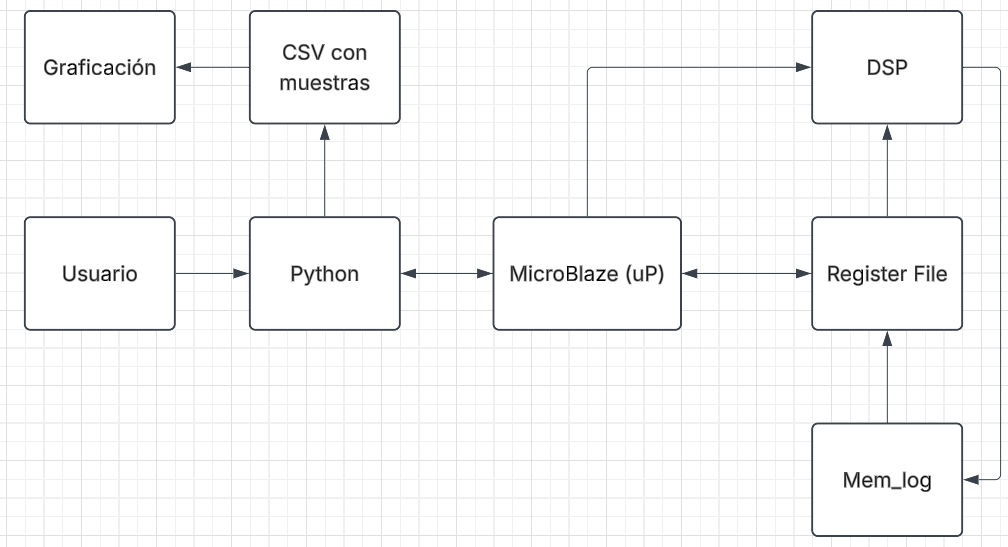
\includegraphics[width=0.7\textwidth]{imagenes/comms_blocks.png}
    \caption{Diagrama en bloques de la comunicación de la implementación.}
    \label{fig:comms_blocks}
\end{figure}

Los bloques principales que componen el sistema son los siguientes:

\begin{itemize}
    \item \textbf{MicroBlaze:} Este bloque se encarga del control de la información mediante el firmware cargado.
    \item \textbf{Procesamiento digital de señales (DSP):} Este bloque es el encargado de realizar el procesamiento de la información generada por la PRBS9, aplicada a un filtro polifásico RC y analizada
    mediante un ber counter.
    \item \textbf{Mem\_log:} Este bloque está compuesto por una BRAM, permite almacenar muestras provenientes de la salida del filtro.
    \item \textbf{Register File:} Finalmente, este bloque se encarga de manejar los comandos enviados por el microprocesador y la información proveniente del DSP de la BRAM.
\end{itemize}

\newpage

\section{Desarollo}
Se dividirá el desarrollo del informe en 6 secciones, 5 de ellas explicando cada bloque funcional por separado, dejando la última sección para la muestra de resultados obtenidos.
    \subsection{Módulo FPGA}
        Este bloque se encarga de la integración a nivel global, instancia los 4 bloques funcionales del sistema, siguiendo el esquema provisto en la figura \ref{fig:comms_blocks}. Además, contiene la codificación del
        bloque MicroGPIO, el cual a su vez contiene el bloque del \textbf{MicroBlaze}, el \textbf{UART} y el \textbf{AXI GPIO}, exportados mediante el IP Block Design.
        
        Expone hacia el resto del diseño el puerto de salida GPO0 de 32 bit, el puerto de entrada GPI0 y la señal locked del clocking wizard, que sirve como reset general del sistema.
        También posee un clocking wizard encargado de generar el clock de 100MHz que se usa a nivel global.

        Como consigna se tuvo que realizar un cambio respecto a la implementación del laboratorio Nº5, donde se utilizaban los leds como lectura del estado de los switches. En este caso, se utilizan
        \texttt{out\_leds[0]} para la señal locked, \texttt{out\_leds[1],[2],[3]} para reflejar el estado del reset, la habilitación de la transmisión y la habilitación de la recepción. De igual manera, 
        se utilizaron los leds RGB para describir el estado de la memoria y de la fase seleccionada, siendo \texttt{RGB0} para la memoria y \texttt{RGB1} para la fase y la indicación de ber nula por fase.

    \subsection{Módulo RF (register\_file)}
        Este bloque contiene un banco de registros de propósito general, que se utilizan dentro del diseño para controlar las variables, acciones y flags del sistema de comunicaciones que existe entre los módulos.
        Implementa el almacenamiento de los comandos como se muestra en la siguiente figura.
        \begin{figure}[H]
            \centering
            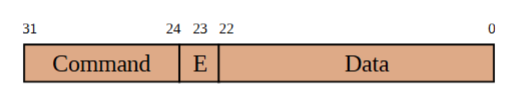
\includegraphics[width=0.7\textwidth]{imagenes/GPIO_output.png}
            \caption{Particionado de bits de salida del GPIO.}
            \label{fig:GPIO_output}
        \end{figure}
        
        El proceso de escritura lo lleva a cabo el procesador, el cual escribe 3 veces el puerto de salida con el mismo comando e información, cambiando solamente el bit de habilitación.
        Este bit de habilitación tiene la importante tarea de avisarle al registro si el dato recibido es confiable o no.

        La primera vez que se escribe la información en el puerto de salida del procesador, el bit de enable se encuentra en 0. El registro lo recibe y espera una nueva muestra, la cuál debería venir con el
        bit de enable en 1. Finalmente, la última muestra se recibe nuevamente con el bit de enable en 0. 
        De esta manera se puede hacer la verificación del comando, dado que si hay cualquier tipo de ruido en la comunicación la señal podría llegar tergiversada.

        Los tipos de comandos dependerán de lo que se desee realizar por el usuario, por lo que queda a libre interpretación del diseñador, para este trabajo se implementaron
        los siguientes comandos:
        \begin{itemize}
            \item \textbf{o\_rst:} Envía un reset generalizado.
            \item \textbf{o\_enb\_tx:} Habilitación de la transmisión.
            \item \textbf{o\_enb\_rx:} Habilitación de la recepción.
            \item \textbf{o\_run\_log:} Activar escritura de la memoria.
            \item \textbf{o\_read\_log:} Leer memoria.
            \item \textbf{o\_addr\_log\_to\_mem:} Dirección de memoria específica.
            \item \textbf{o\_rd\_sel:} Seleccionar el código a leer.
            \item \textbf{o\_ber\_rst:} Reset de contadores de BER. (Implementado por un error en el diseño provisto en el Lab.Nº4, donde la BER solo se reseteaba al cambiar de fase.)
        \end{itemize}
    \subsection{Módulo BRAM (mem\_log)}    
        Representa la implementación de la BRAM, con una capacidad de 32K x 32b. La escritura de la memoria se activa mediante el flanco ascendente del comando
        \textbf{o\_run\_log}, de tal manera que la memoria llena sus casillas a una velocidad de clock. Una vez la memoria se llena, se detiene la escritura y se activa la flag
        \textbf{i\_mem\_full}, que como su nombre indica, avisa que la memoria está llena y lista para la lectura.

        Por el contrario, el proceso de lectura usa \textbf{o\_addr\_log\_to\_mem} como dirección y \textbf{o\_read\_log} como comando de habilitación. Una vez llega el comando
        de habilitación, el dato solicitado se carga y se envía por medio de \textbf{i\_data\_log\_from\_mem}.

        Algo importante a tener en cuenta es que la lectura se bloquea al escribir para evitar errores graves de pérdida de información, siendo este bloqueo controlado por el firmware del MicroBlaze,
        donde deshabilita \textbf{o\_read\_log} antes de que la memoria envíe datos.
    \subsection{Módulo DSP (dsp\_core)}
        Finalizando con los módulos de verilog, no hay mucho de este módulo que no se haya comentado ya en anteriores laboratorios, consiste de los siguientes sub-módulos:
        \begin{itemize}
            \item \textit{PRBS9:} Genera una secuencia pseudoaleatoria de 9 bits. Tiene 2 instancias, una para los datos de entrada del upscaling y otro para
            la generación de la referencia para el contador de BER.
            \item \textit{control:} Encargado de decodificar las señales provenientes del Register File, como ser \texttt{en\_tx, en\_rx y phase\_sw}. A su vez, resetea
            el contador de BER al detectar un cambio de fase.
            \item \textit{freq\_divider:} Genera la base de tiempo que utiliza el banco de coeficientes del filtro polifásico para aplicar el filtrado de los bits enviados
            por la PRBS9.
            \item \textit{rc\_tx:} Contiene el filtro polifásico de coseno realzado (RC) junto con sus coeficientes. Este módulo recibe el selector de fase proveniente del \textit{freq\_divider} que
            funciona como selector, de tal manera entrega cuatro muestras interpoladas por símbolo. Finalmente, se  aplica una sumatoria de cada tap según el bit almacenado en el registro de desplazamiento.
            \item \textit{decimator:} Como su mismo nombre lo indica, se encarga de tomar una muestra por símbolo según la fase seleccionada, también actúa como slicer para quedarse con el bit de signo.
            \item \textit{ber\_counter:} Por medio de la PRBS9, compara los bits enviados desde el \textit{decimator} con los generados por cada semilla. Dado que se debe hacer la comparación correcta, la referencia tiene que estar alineada
            con el retardo de la cadena total. También es destacable la implementación de una compensación para el cambio de fase.
        \end{itemize}

    \subsection{Firmware del MicroBlaze}
        Escrito en \textbf{lenguaje C}, se encarga de hacer de intérprete entre las tramas enviadas por UART y el GPIO.
        El bucle principal de funcionamiento espera un header válido de iniciación y uno válido de finalización, para luego enviar los datos según el device seleccionado. Es importante destacar que
        en caso de no obtener una igualdad entre el header esperado (101+L/S+Size) y el recibido se realizará el descarte de la trama completa. Lo mismo ocurre para el trailer esperado (010+L/S+Size) y el recibido.

        Para la lectura de trama, el bit de Size y el tamaño de la información en caso de ser una trama corta deben coincidir tanto en el \textbf{Header} como en el \textbf{Trailer}.

        También implementa el protocolo de escritura de la figura \ref{fig:GPIO_output}, donde arma tramas de 32bits con el comando en la parte alta y el dato en la parte baja, escribiendo 3 veces el puerto GPIO para que
        se cumpla la verificación del bit de enable (Strobing).

        El código pretende abarcar 3 dispositivos, los cuales se detallan a continuación:
        \begin{itemize}
            \item \textbf{DEV\_RF\_WRITE:} Escritura del Register File. Recibe 4 bytes; El comando y el dato. Luego llama al protocolo de strobeo.
            \item \textbf{DEV\_RF\_READ:} Lectura del Register File. Recibe un byte con el código de lectura.
            \item \textbf{DEV\_READ\_SW:} Lectura de los 4 bits de los switches.
        \end{itemize}
    \subsection{Python Script}
        Este script representa la interfaz de usuario, donde se escriben los comandos para controlar el sistema. Consta de tres capas:
        \begin{enumerate}
            \item \textbf{Capa de trama:} Tiene una función encargada de armar la trama y seleccionar el tipo de formato según el tamaño de la información, es decir, distingue entre trama corta
            y trama larga. También consta de otra función que hace lo contrario para los casos donde se necesite recibir datos.
            \item \textbf{Capa de registros:} Construye la lectura y escritura del register file, de tal manera que luego se puede leer el status del registro, leer el dato proporcionado
            por los contadores de BER o leer la salida del filtro Tx.
            \item \textbf{Capa de comandos:} Es la consola que maneja los comandos que permiten exponer cada registro del register file como un comando junto con otras tres operaciones compuestas,
            también encontramos comandos tales como \textit{ber\_sweep}, que mide la BER de las cuatro fases, y \textit{dumplog}, que descarga cierta cantidad de muestras a un archivo .csv para luego
            graficarlas mediante otro script.
        \end{enumerate}
        El script que genera las gráficas del \textit{dumplog} permite visualizar la salida del filtro para cada una de las fases, superponiéndolas
        con las muestras que le toca a cada fase teniendo en cuenta el decimador para la fase seleccionada. Por otro lado, genera un diagrama de ojo para fase y cuadratura.
        
        Los comandos que posee la interfaz de usuario se listan a continuación:
        \begin{itemize}
            \item \texttt{rst <0/1>:} Reset del DSP.
            \item \texttt{entx <0/1> | enrx <0/1>:} Habilitación de transmisión y recepción.
            \item \texttt{phase <0-3>:} Selección de fase.
            \item \texttt{sw:} Lectura de llaves.
            \item \texttt{status:} Lectura de los registros del RF.
            \item \texttt{ber:} Lectura de los contadores de muestras y errores para la fase seleccionada.
            \item \texttt{berrst:} Reset de los contadores de la fase actual.
            \item \texttt{bersweep:} Ber de las cuatro fases.
            \item \texttt{runlog:} Habilitación de carga de memoria.
            \item \texttt{memfull:} Read de flag de memoria llena.
            \item \texttt{addr <n>:} Fija una dirección de memoria
            \item \texttt{readword <n>:} Lee una dirección de memoria.
            \item \texttt{dumplog <n> [archive]:} Guarda n muestras de la memoria a un archivo .csv
            \item \texttt{buildid:} Permite ver la versión actual del bitstream.
            \item \texttt{help:} Relanzar lista de comandos.
            \item \texttt{exit:} Salir de la comunicación.
        \end{itemize}
    \subsection{Resultados obtenidos}
        Comenzando con este apartado, se desea llevar a cabo el proceso de comunicación completo mediante los comandos diseñados.
        Teniendo esto en cuenta, se escribieron los siguientes comandos;
        \begin{figure}[H]
            \centering
            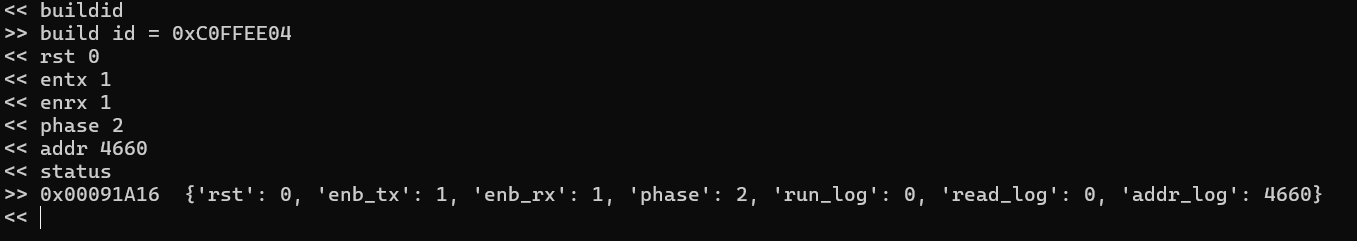
\includegraphics[width=0.7\textwidth]{imagenes/initialize_commands.png}
            \caption{Comandos para inicializar la comunicación}
            \label{fig:initialize_commands}
        \end{figure}
        En la figura \ref{fig:initialize_commands} se pueden ver el funcionamiento de los comandos de inicialización de la comunicación, como ser
        la habilitación de la transmisión y recepción, la selección de fase o el estado del reset. Los cuales se muestran mediante \texttt{status.}
        Consiguientemente, se tiene la seguidilla de comandos que permiten ver la BER para una fase en específico.
        \begin{figure}[H]
            \centering
            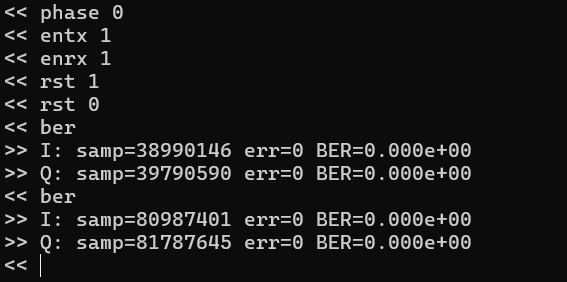
\includegraphics[width=0.7\textwidth]{imagenes/phase0_ber_visualize.png}
            \caption{BER para la fase 0.}
            \label{fig:phase0_ber_visualize}
        \end{figure}
        Lo mismo se puede plantear para todas las fases, obteniendo las siguientes lecturas.
        \begin{figure}[H]
            \centering
            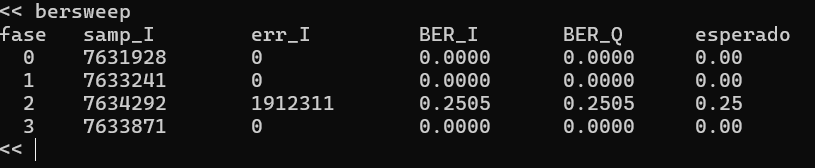
\includegraphics[width=0.7\textwidth]{imagenes/bersweep_I_Q.png}
            \caption{BER de todas las fases.}
            \label{fig:bersweep_I_Q}
        \end{figure}
        En lo que respecta a la RAM, las siguientes imágenes muestran la escritura y lectura.
        \begin{figure}[H]
            \centering
            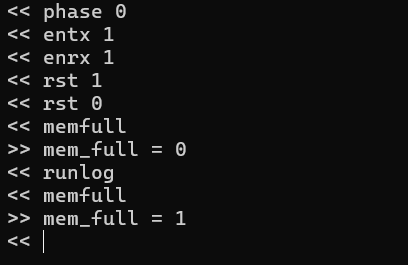
\includegraphics[width=0.5\textwidth]{imagenes/mem_log_try.png}
            \caption{Escritura de la RAM.}
            \label{fig:mem_log_try}
        \end{figure}
        \begin{figure}[H]
            \centering
            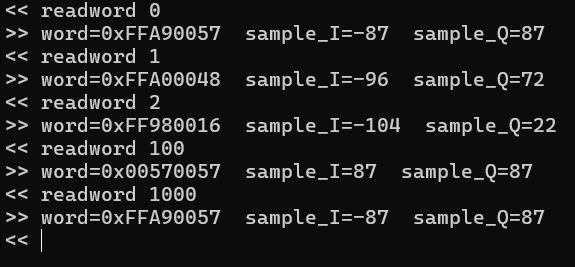
\includegraphics[width=0.7\textwidth]{imagenes/mem_log_readings.png}
            \caption{Lectura de la RAM.}
            \label{fig:mem_log_readings}
        \end{figure}
        La carga de datos al archivo .csv permite generar los siguientes gráficos, tomando como referencia a la fase 0 a la hora de la carga.
        \begin{figure}[H]
            \centering
            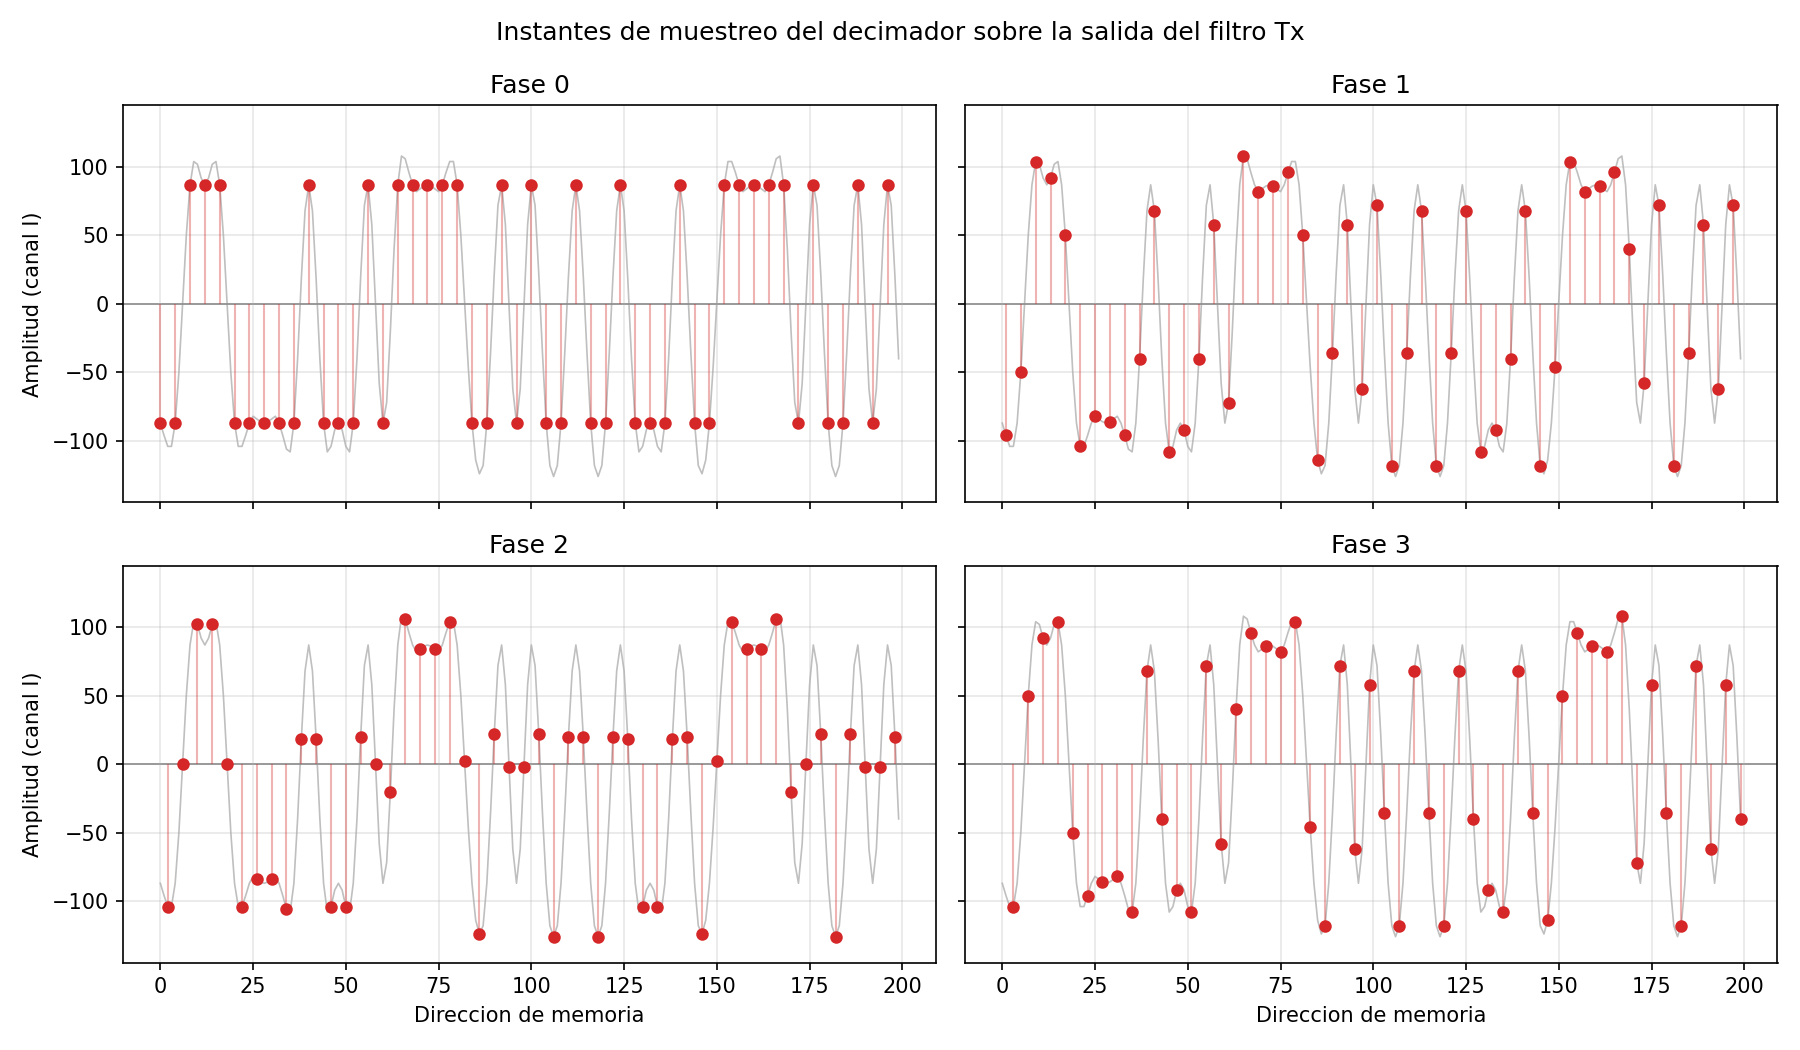
\includegraphics[width=0.7\textwidth]{imagenes/log_fase0_fases.png}
            \caption{Salida filtro Tx para todas las fases.}
            \label{fig:log_fase0_fases}
        \end{figure}
        \begin{figure}[H]
            \centering
            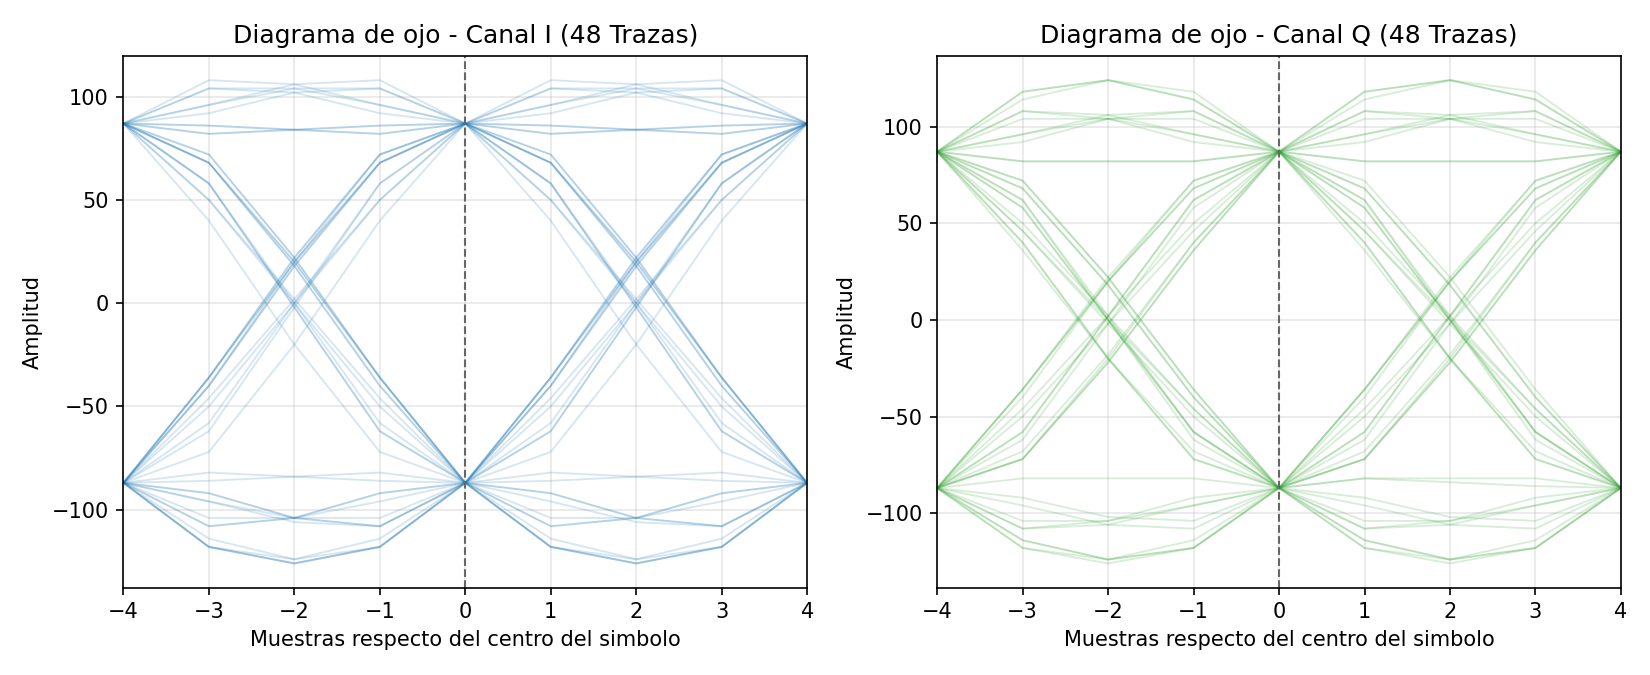
\includegraphics[width=0.7\textwidth]{imagenes/log_fase0_ojos.png}
            \caption{Diagrama de ojos de fase y cuadratura.}
            \label{fig:log_fase0_ojos}
        \end{figure}
        Por último, el comando de lectura de los switches se puede ver a continuación.
        \begin{figure}[H]
            \centering
            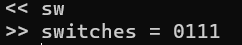
\includegraphics[width=0.4\textwidth]{imagenes/sw_command.png}
            \caption{Lectura de switches.}
            \label{fig:sw_command}
        \end{figure}

\newpage

\section{Conclusiones}
    Finalizando este informe, se concluye que el sistema funciona debidamente, y comparando con los resultados obtenidos de la salida del filtro y el diamagra de ojos,
    con los esperados según las simulaciones realizadas en punto fijo de laboratorios anteriores, la salida obtenida es de buena calidad. De igual manera, la implementación de la memoria
    y de la interfaz de usuario permite un espacio más amigable para el control del sistema, evitando el uso de VIO e ILA para este caso concreto.
    
    Las mayores dificultades se obtuvieron con Vitis, donde la imposibilidad de switchear el archivo .xsa (Exportación del Hardware desde Vivado), generó la necesidad de crear
    un comando que permita ver la versión actual del bitstream y evitar así interpretaciones erróneas.
\end{document}